\documentclass[11pt]{article}
\usepackage[utf8]{inputenc}
\usepackage{xspace}
\usepackage[usenames]{xcolor}
\usepackage{listings}
\usepackage[absolute]{textpos}
\usepackage[many]{tcolorbox}
\usepackage{geometry}
\usepackage[colorlinks = true]{hyperref}

\usepackage{natbib}
\usepackage{graphicx}

\usepackage{multirow}
\usepackage{tabularx}
\usepackage{booktabs}

\definecolor{green}{rgb}{0.13, 0.55, 0.13}
\definecolor{fscolor}{RGB}{44,118,255}

\lstset{breaklines=true,
  breakatwhitespace=true,
  stepnumber=1,
  basicstyle=\ttfamily\footnotesize,
  commentstyle=\ttfamily\color{gray}\textit\footnotesize,
  prebreak={\textbackslash},
  breakindent=10pt,
  breakautoindent=false,
  showspaces=false,
  showstringspaces=false,
  frame=single,
  rulesepcolor=\color{gray},
  rulesep=0.1em,
  abovecaptionskip=0em,
  aboveskip=1.5em,
  belowcaptionskip=0.5em,
  belowskip=1em,
  keywordstyle=\color{green},
  escapeinside={(*}{*)},
  language=C++
}

\lstset{emph={%
 override%
  },emphstyle={\color{red}}%
}%
\newcommand{\code}[1]{\lstinline[breaklines=true,breakatwhitespace=false,postbreak=,prebreak=,breakindent=0pt]{#1}}
\newcommand{\cbs}{\code{CBS}\@\xspace}
\newcommand{\ma}{\code{MA5}\@\xspace}
\newcommand{\mg}{\code{MadGraph5_aMC@NLO}\@\xspace}
\newcommand{\cm}{\code{CM2}\@\xspace}
\newcommand{\de}{\code{Delphes}\@\xspace}
\newcommand{\ana}{ATLAS\_13TeV\_0LEP\_139invfb\@\xspace}

\newcommand{\gev}{\ensuremath{\,\text{GeV}}}
\newcommand{\tev}{\ensuremath{\,\text{TeV}}}

\newcommand{\figref}[1]{\figurename~\ref{#1}}
\newcommand{\subfigref}[1]{(\subref{#1})}
\newcommand{\secref}[1]{Section~\ref{#1}}
\newcommand{\appref}[1]{Appendix~\ref{#1}}
\newcommand{\tabref}[1]{\tablename~\ref{#1}}
\newcommand{\exref}[1]{Example~\ref{#1}}
\newcommand{\refeqs}[1]{Eq.s~\ref{#1}}
\newcommand{\refcite}[1]{Ref.~\cite{#1}}
\newcommand{\refapp}[1]{App.~\ref{#1}}


\title{CBS\_ATLAS\_13TeV\_0LEP\_139invfb}
\author{Yang Zhang}
\date{June 2020}

\begin{document}

\maketitle

We present here the cut-flows of the analysis \ana~\cite{ATLAS-CONF-2019-040} obtained from \cbs~(ColliderBIT\_Solo), \ma~(MadAnalysis~5) and \cm~(CheckMATE~2). The analysis aims to search for squarks and gluinos in final states containing jets and missing transverse momentum at 13 TeV LHC, corresponding to an integrated luminosity of 139 fb$^{-1}$. There are two approaches used in this analysis, ‘multi-bin search’ and ‘BDT search’. In all the tools, only the ‘multi-bin search’ signal regions (SRs) are implemented. 

There are ten cut-flows provided in Table 16, 17 and 18 of \cite{ATLAS-CONF-2019-040}. Here we choose one cut-flow from each table to compare the cut-flows of different tools, which are 
\begin{itemize}
    \item Squark-pair production, followed by the direct decays of squarks, $\widetilde{q}\to q\widetilde{\chi}_1^0$, with $(m_{\widetilde{q}} = 1200 \gev,m_{\widetilde{\chi}_1^0}=600 \gev)$. In following, we call it SS direct model point.
    \item Gluino-pair production, followed by the direct decays of gluinos, $\widetilde{g}\to qq\widetilde{\chi}_1^0$, with $(m_{\widetilde{g}} = 1400 \gev,m_{\widetilde{\chi}_1^0}=1000 \gev)$. In following, we call it GG direct model point. 
    \item Gluino-pair production, followed by one-step cascade decays of gluinos, $\widetilde{g}\to q\widetilde{\chi}_1^\pm \to qW^\pm\widetilde{\chi}_1^0$, with $(m_{\widetilde{g}} = 1400 \gev,m_{\widetilde{\chi}_1^\pm}=1100 \gev, m_{\widetilde{\chi}_1^0}=800 \gev)$. In following, we call it GG one-step model point. 
\end{itemize}
All other supersymmetric particles have their masses set such that the particles are effectively decoupled. Direct decays are those where the squarks or gluinos decay directly into SM particles and the $\widetilde{\chi}_1^0$, while the one-step decays refer to the cases where the decays occur via one intermediate on-shell SUSY particle. Eightfold degeneracy of first- and second-generation squarks is assumed for the simplified models with direct decays of squarks. The gluino is allowed to decay into four flavors (u,d,s,c) of quarks in simplified models with gluino-pair production.

\section{SS direct model point}

\subsection{Leading-order events}

Firstly, we use \code{ColliderBIT} to generate events for the SS direct model point, which essentially uses the LO Pythia generator. The cut-flows obtained from \cbs, \ma and \ma are shown in \tabref{tab:ss_direct_pythia} and \figref{fig:ss_direct_pythia}.

\begin{table}[t]
\small
\begin{tabularx}{\textwidth}{llllll}
\toprule
                         &                                                & ATLAS                 & CBS                      & CM                       & MA5                      \\
\midrule
                         & No cut                                         &                       & 2552.90                  & 2439.80                  & 2435.51                  \\
                         & Pre-sel$+E_T^{miss}>300\gev$                   & \multirow{2}{*}{1763} & \multirow{2}{*}{1763.00} & \multirow{2}{*}{1763.00} & \multirow{2}{*}{1763.00} \\
                         & $+p_T(j_1)>200\gev+m_{eff}>800\gev$             &                       &                          &                          &                          \\
                         & $N_j \leq2$                                    & 1763                  & 1743.00                  & 1763.00                  & 1763.00                  \\
                         & Cleaning                                       & 1746                  & 1707.71                  &                          &                          \\
\midrule
\multirow{6}{*}{2j-1600} & $\Delta\phi(j_{1,2,(3)},P_T^{miss})_{min}>0.8$ & 1433                  & 1387.13                  & 1428.21                  & 1424.70                  \\
                         & $\Delta\phi(j_{i>3},P_T^{miss})_{min}>0.4$     & 1377                  & 1322.25                  & 1361.80                  & 1360.07                  \\
                         & $p_T(j_2)>250\gev$                             & 853                   & 826.81                   & 805.33                   & 778.41                   \\
                         & $|\eta(j_{1,2})|<2.0$                          & 835                   & 808.29                   & 785.96                   & 760.84                   \\
                         & $E_T^{miss}/\sqrt(H_T)>16\gev^{1/2}$           & 568                   & 541.33                   & 513.58                   & 500.30                   \\
                         & $m_{eff}>1600\gev$                             & 366                   & 366.71                   & 329.81                   & 316.06                   \\
\midrule
\multirow{5}{*}{2j-2200} & $\Delta\phi(j_{1,2,(3)},P_T^{miss})_{min}>0.4$ & 1603                  & 1552.35                  & 1597.00                  & 1598.52                  \\
                         & $\Delta\phi(j_{i>3},P_T^{miss})_{min}>0.2$     & 1567                  & 1513.22                  & 1555.47                  & 1559.10                  \\
                         & $p_T(j_1)>600\gev$                             & 509                   & 489.70                   & 465.90                   & 439.03                   \\
                         & $E_T^{miss}/\sqrt(H_T)>16\gev^{1/2}$           & 337                   & 323.45                   & 304.78                   & 290.47                   \\
                         & $m_{eff}>2200\gev$                             & 101                   & 96.32                    & 85.00                    & 78.88                    \\
\midrule
\multirow{6}{*}{2j-2800} & $\Delta\phi(j_{1,2,(3)},P_T^{miss})_{min}>0.8$ & 1433                  & 1387.13                  & 1428.21                  & 1424.70                  \\
                         & $\Delta\phi(j_{i>3},P_T^{miss})_{min}>0.4$     & 1377                  & 1322.25                  & 1361.80                  & 1360.07                  \\
                         & $p_T(j_2)>250\gev$                             & 853                   & 826.81                   & 805.33                   & 778.41                   \\
                         & $|\eta(j_{1,2})|<1.2$                          & 655                   & 626.86                   & 610.19                   & 591.06                   \\
                         & $E_T^{miss}/\sqrt(H_T)>16\gev^{1/2}$           & 439                   & 419.17                   & 398.52                   & 388.04                   \\
                         & $m_{eff}>2800\gev$                             & 15.6                  & 13.85$_{\pm0.8}$            & 11.76$_{\pm0.76}$           & 10.37$_{\pm0.71}$ \\
\bottomrule
\end{tabularx}
\caption{Cut-flows for SS direct model point with events generated by \code{ColliderBIT}. The number of events obtained with \cbs, \cm and \ma after the Pre-sel$+E_T^{miss}+p_T(j_1)+m_{eff}$ cut are scaled to such number of the ATLAS table. The errors added in the bottom row are statistical errors.}
\label{tab:ss_direct_pythia}
\end{table}

\begin{figure}[p]
\centering
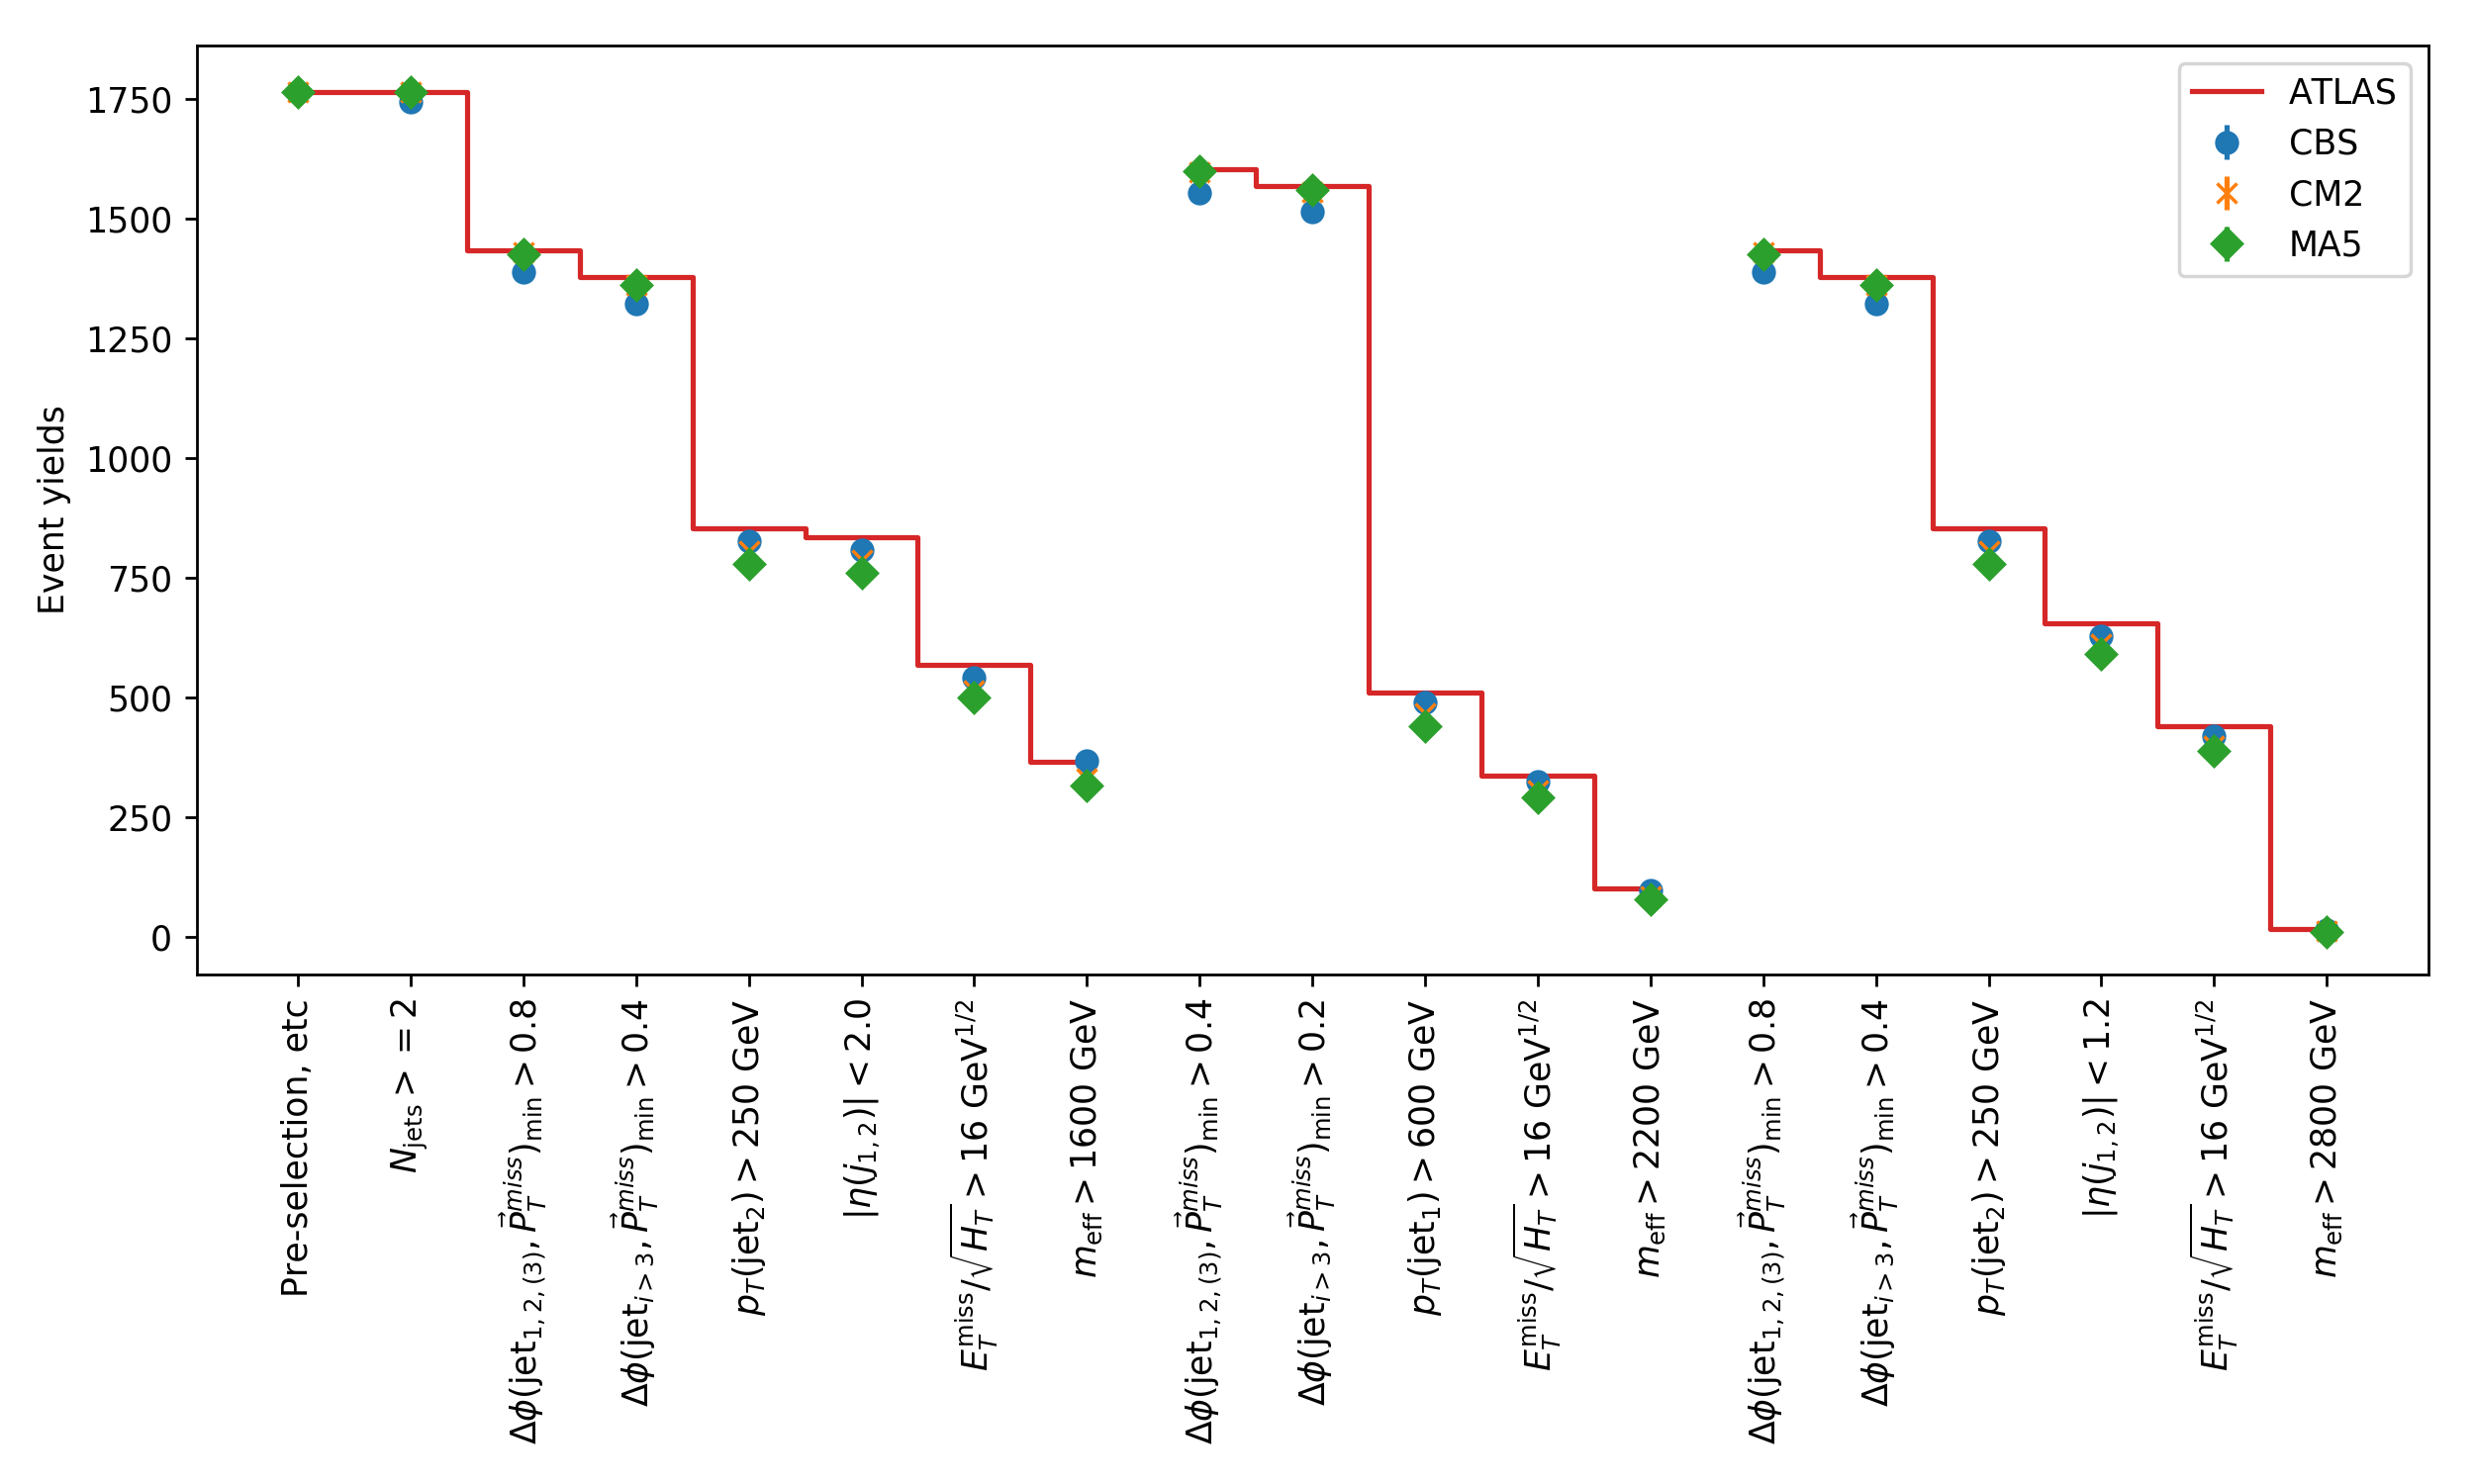
\includegraphics[width=.9\textwidth]{fig/no2j_tab_16.png}\\
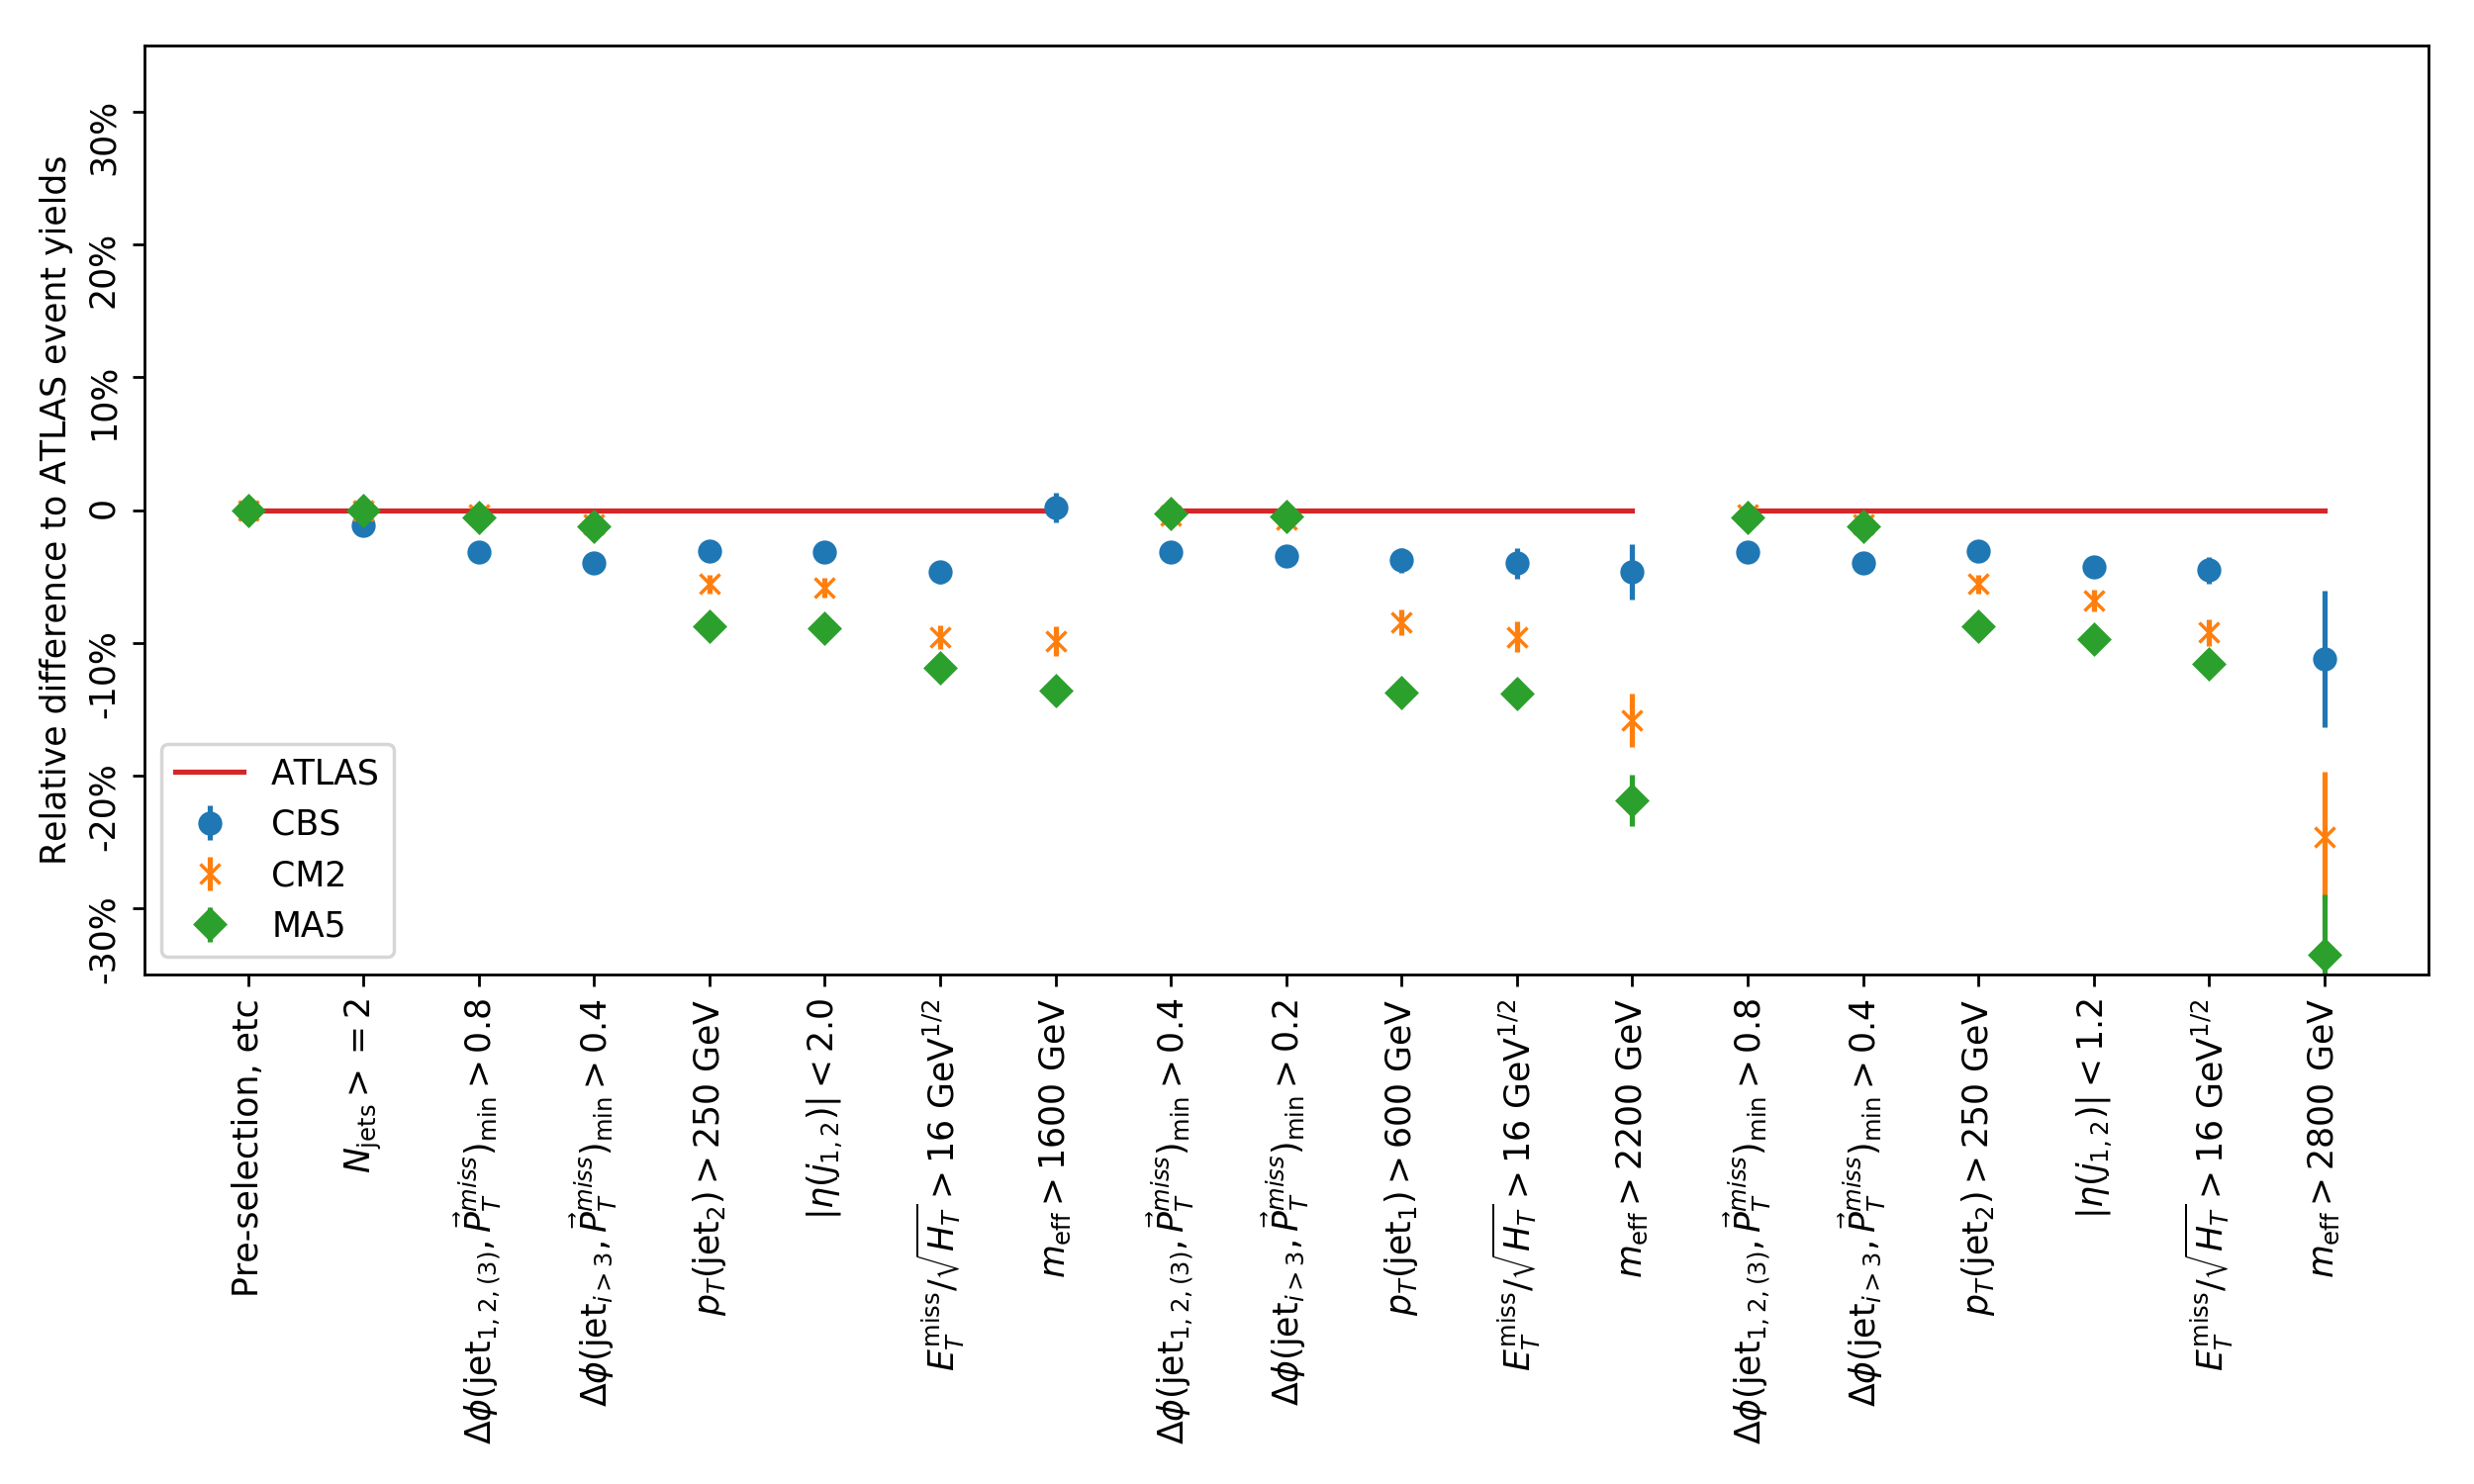
\includegraphics[width=.9\textwidth]{fig/no2j_norm_tab_16.png}
\caption{Cut-flows for SS direct model point with events generated by \code{ColliderBIT}. Upper: y-axis shows the event yields in \tabref{tab:ss_direct_pythia} directly. Lower: y-axis shows the relative difference to ATLAS event yields.}
\label{fig:ss_direct_pythia}
\end{figure}

The number of events obtained with \cbs, \cm and \ma after the Pre-sel$+E_T^{miss}+p_T(j_1)+m_{eff}$ cut are scaled to such number of the ATLAS table. The relative difference to ATLAS event yields shown in the lower panel of \figref{fig:ss_direct_pythia} is defined as 
\begin{equation}
 R_i = \frac{N_i-N_i^{\rm ATLAS}}{N_i^{\rm ATLAS}}
\end{equation}
where $N_i$ is number of events after each cut in the \cbs, \cm and \ma cut-flows, and $N_i^{\rm ATLAS}$ indicates number of events in the ATLAS cut-flow.

All the three generated cut-flows are consistent with the ATLAS with in 30\% deviation. In general, \cbs obtains the best agreement. The most conspicuous discrepancies among cut-flows of \cbs, \cm and \ma start from the cut of $P_T(jet_2)>250\gev$ or $P_T(jet_1)>600\gev$. Obviously, it is caused by the jets reconstruction in different tools. 


\begin{figure}[ht]
\centering
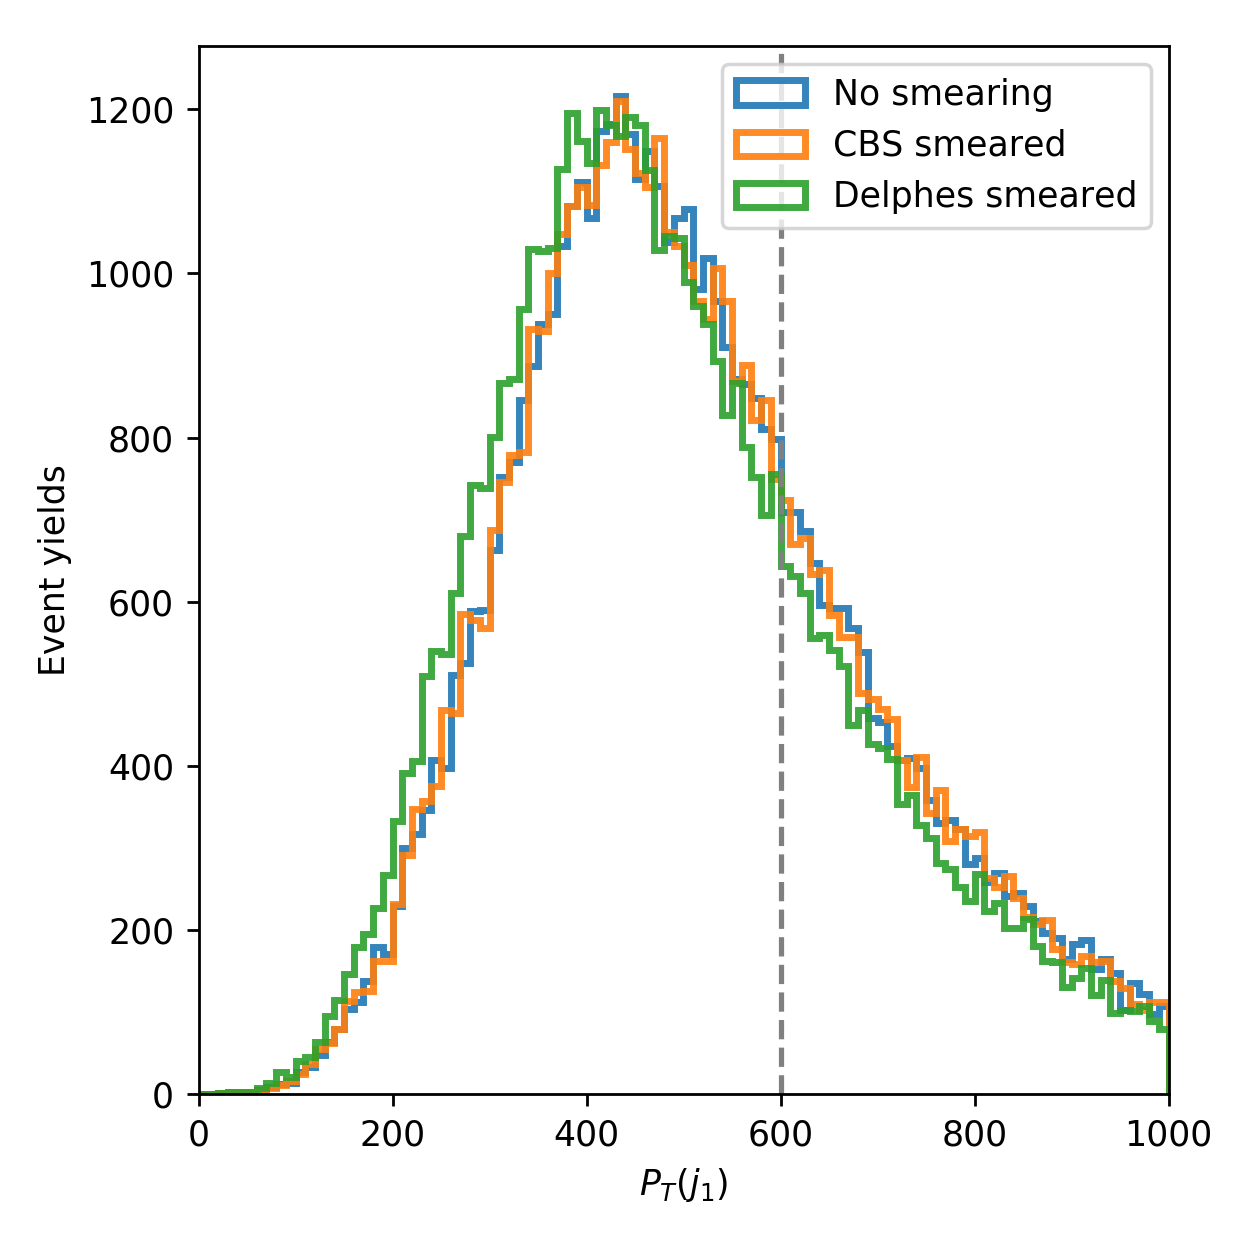
\includegraphics[width=.48\textwidth]{fig/P_T(j_1).png} 
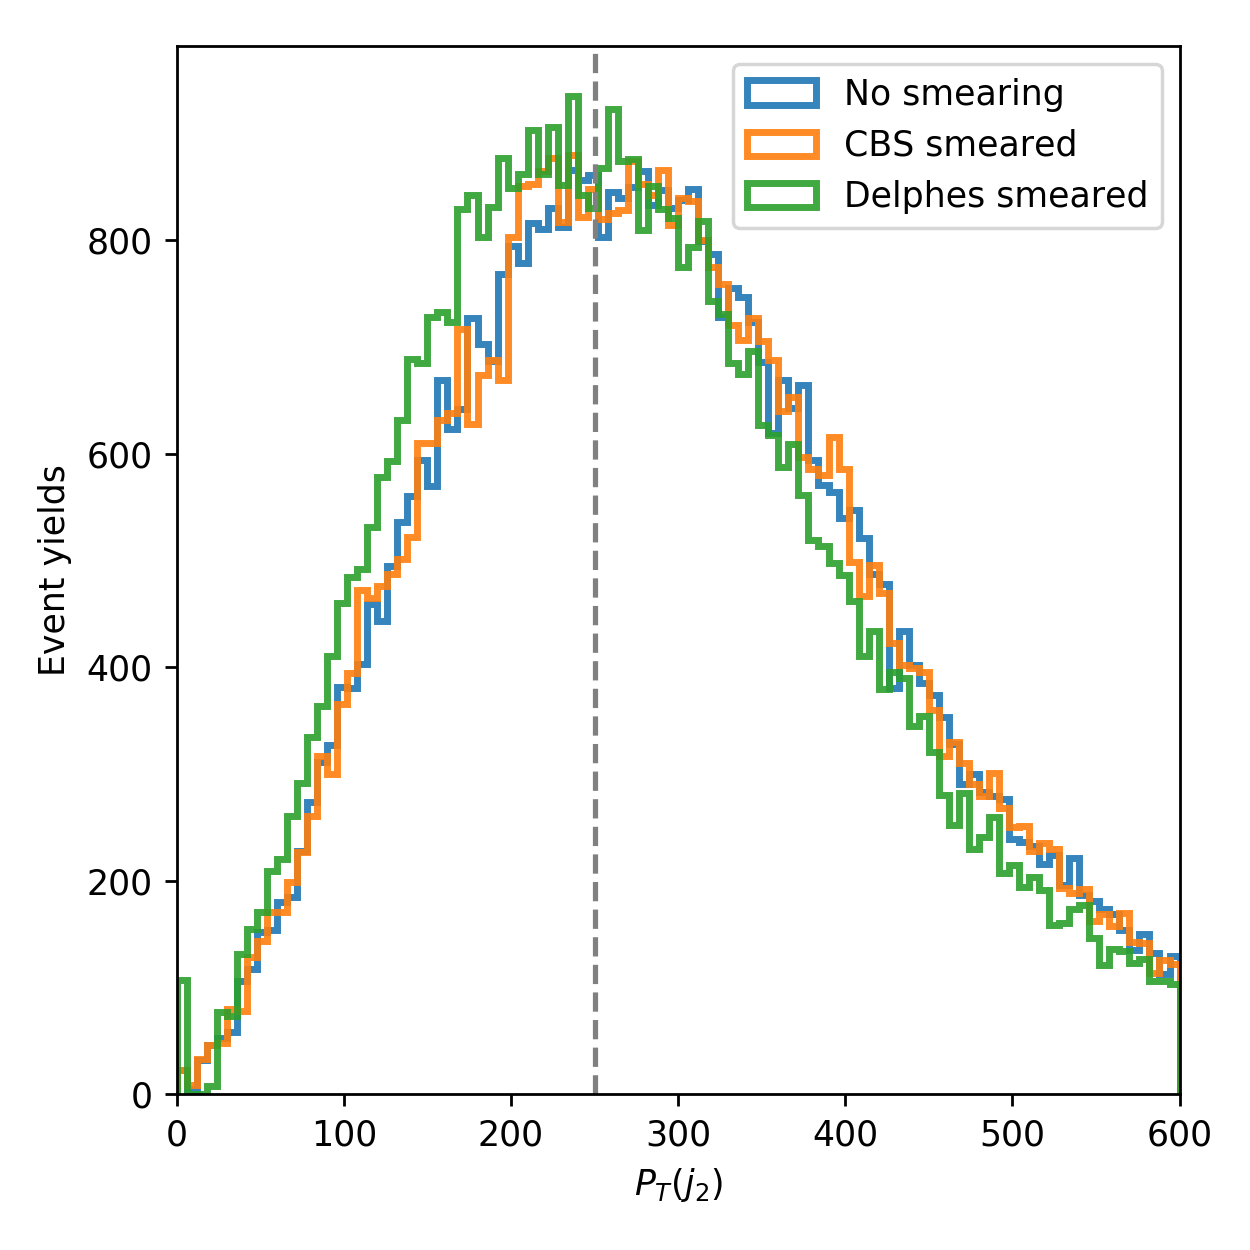
\includegraphics[width=.48\textwidth]{fig/P_T(j_2).png}
\caption{Distribution of $P_T$ of jets reconstructed in \cbs and \de. Jets without smearing are exactly same in \cbs and \de. }
\label{fig:jet_smear}
\end{figure}

In \figref{fig:jet_smear}, we present $P_T$ of jets reconstructed in \cbs and \de. As for \de, we adopt the \de card used for \ana of \ma (which is called ATLAS-CONF-2019-040 in \ma). We have checked that the un-smeared jets from \cbs and \de are exactly same. The smearing functions in \cbs basically maintain the distribution functions of momentum of jets, while $P_T$ of jets are reduced in \ma. Besides, some of the jets in \de are discarded due to jet flavor association checking. As a result, less events in \ma pass the cut of $P_T(jet_2)>250\gev$ or $P_T(jet_1)>600\gev$.


\begin{figure}[ht]
\centering
\includegraphics[width=.48\textwidth]{fig/E_T^{miss}.png} 
\includegraphics[width=.48\textwidth]{fig/M_{eff}.png}
\caption{Distribution of $E_{T}^{miss}$ (left) and $m_{eff}$ (right) obtained in \cbs and \de. $E_{T}^{miss}$ is not smeared in \cbs. }
\label{fig:meff_smear}
\end{figure}

The smearing in \ma also decrease the $E_{T}^{miss}$, as shown in \figref{fig:meff_smear}, while \cbs uses un-smeared $E_{T}^{miss}$. Thus, the Pre-sel$+E_T^{miss}+p_T(j_1)+m_{eff}$ cut rejects more event in \ma than in \cbs. However, we scaled the number of events after that cut to the ATLAS one, so it lead to slightly more events in the following cuts in \ma and \cm. Furthermore, because the $m_{eff}$ is defined to be the scalar sum of $E_{T}^{miss}$ and the transverse momenta of all jets with $p_T>50\gev$, there are more events of low $m_{eff}$ in \ma than that in \cbs. As a result, less events in \ma pass the cut of $m_{eff}>1600,~2200,~2800\gev$.

\subsection{Events with up to 2 extra jets}

To be fair to \ma, we further generate event in the way described in \ma validation note~\cite{Ambrogi}. The events are generated using \mg with the inclusion of up to 2 additional extra jets. Then the events are showered and hadronized using \code{Pythia8}. The matching and merging between the matrix element and the parton shower formalism is performed by the script \code{main89.cc} of \code{Pythia8}, using the CWKKL algorithm. The merging scale is set to 1/4 of the mass of the gluino or squark up to the value of $500\gev$. The cut-flows obtained from \cbs, \ma and \ma are shown in \tabref{tab:ss_direct_merging} and \figref{fig:ss_direct_merging}.



\cite{Araz:2020lnp}

\newpage

\section{GG direct model point}


\section{GG one-step model point}


\bibliography{refs}
\bibliographystyle{plain}

\end{document}
